%---------------------------------------------------------------------------------------------------------------
% TEMPLATE PARA TRABALHO DE CONCLUSÃO DE CURSO
% Instituto Federal de Educação, Ciência e Tecnologia de São Paulo - IFSP
% Campus Campinas
%
% Baseado no trabalho de Michael Vornes (https://github.com/mvornes).
% 
% Autor: Daniel Brai
% Ano: 2022
% 
%----------------------------------------------------------------------------------------------------------------
% Codificação: UTF-8
% LaTeX:  abnTeX2          
% ---------------------------------------------------------------------------------------------------------------


% CARREGA CLASSE PERSONALIZADA-----------------------------------------------------------------------------------
\documentclass[%twoside,                   % Impressão em frente e verso
    	        oneside,                   % Impressão apenas frente
]{configuracoes/ifsp_campinas-abntex2}

% DADOS DO ALUNO--------------------------------------------------------------------------------------------------
\autor{Daniel Brai Gonzales Marcos}
\autorcitacao{BRAI, Daniel} 
\numeroRA{3013375}
% DADOS DO CURSO
\curso{Ciência de Dados}
\modalidadecurso{Pós-Graduação}
\data{2022}
% DADOS DA INSTITUIÇÃO--------------------------------------------------------------------------------------------
\campus{Campinas}
\cidade{Campinas}
\instituicao{Instituto Federal de Educação, Ciência e Tecnologia de São Paulo}
\programa{curso de Pós Graduação em Informática Aplicada a Educação}
%\logoinstituicao{0.2}{dados/figuras/logo-instituicao.png} 
% DADOS DOS ORIENTADORES------------------------------------------------------------------------------------------
%\orientador{Prof. Me. Danilo Camargo Bueno}
%\instOrientador{Universidade Estadual de Maringá - UEM}
%\orientador[Orientadora:]{Nome da orientadora}
% DADOS DO TRABALHO-----------------------------------------------------------------------------------------------
\titulo{Análise da Aplicabilidade de Técnicas de NLP e de \textit{Clustering} para Segmentação de Cartas do \textit{Jogo Magic: The Gathering}}
\titleabstract{Article's Title here}
\tipoprojeto{Projeto de Pesquisa}

% INCLUI ARQUIVOS DE CONFIGURAÇÕES-------------------------------------------------------------------------------
% REFERÊNCIAS------------------------------------------------------------------
\usepackage[%
    alf,
    abnt-emphasize=bf,
    bibjustif,
    recuo=0cm,
    abnt-url-package=url,       % Utiliza o pacote url
    abnt-refinfo=yes,           % Utiliza o estilo bibliográfico abnt-refinfo
    abnt-etal-cite=3,
    abnt-etal-list=3,
    abnt-thesis-year=final
]{abntex2cite}                  % Configura as citações bibliográficas conforme a norma ABNT

% PACOTES----------------------------------------------------------------------
\usepackage[utf8]{inputenc}                                 % Codificação do documento
\usepackage{fontenc}                                 % Seleção de código de fonte
\usepackage{booktabs}                                       % Réguas horizontais em tabelas
\usepackage{color, colortbl}                                % Controle das cores
\usepackage{float}                                          % Necessário para tabelas/figuras em ambiente multi-colunas
\usepackage{graphicx}                                       % Inclusão de gráficos e figuras
\usepackage{icomma}                                         % Uso de vírgulas em expressões matemáticas
\usepackage{indentfirst}                                    % Indenta o primeiro parágrafo de cada seção
\usepackage{microtype}                                      % Melhora a justificação do documento
\usepackage{multirow, array}                                % Permite tabelas com múltiplas linhas e colunas
\usepackage{subeqnarray}                                    % Permite subnumeração de equações
\usepackage{lastpage}                                       % Para encontrar última página do documento
\usepackage{verbatim}                                       % Permite apresentar texto tal como escrito no documento, ainda que sejam comandos Latex
\usepackage{amsfonts, amssymb, amsmath}                     % Fontes e símbolos matemáticos
\usepackage[algoruled, portuguese]{algorithm2e}             % Permite escrever algoritmos em português
%\usepackage[scaled]{helvet}                                % Usa a fonte Helvetica
\usepackage{times}                                          % Usa a fonte Times
%\usepackage{mathptmx}
%\usepackage{palatino}                                      % Usa a fonte Palatino
%\usepackage{lmodern}                                       % Usa a fonte Latin Modern
\usepackage[bottom]{footmisc}                               % Mantém as notas de rodapé sempre na mesma posição
\usepackage{ae, aecompl}                                    % Fontes de alta qualidade
\usepackage{latexsym}                                       % Símbolos matemáticos
\usepackage{lscape}                                         % Permite páginas em modo "paisagem"
%\usepackage{picinpar}                                      % Dispor imagens em parágrafos
%\usepackage{scalefnt}                                      % Permite redimensionar tamanho da fonte
%\usepackage{subfig}                                        % Posicionamento de figuras
%\usepackage{upgreek}                                       % Fonte letras gregas

\usepackage{stringstrings}                                  % Capitalização

\usepackage{multido}
\usepackage{xparse, etoolbox}

\usepackage{pgfplots}
\usepackage{filecontents}

\usepackage{venndiagram}

\usepackage{nameref}

\usepackage{hyperref}
\usepackage{cleveref}

% Redefine a fonte para uma fonte similar a Arial (fonte Helvetica)
\renewcommand*\familydefault{\sfdefault}

% CONFIGURAÇÕES DE APARÊNCIA DO PDF FINAL--------------------------------------
\makeatletter
\hypersetup{%
    portuguese,
    colorlinks=true,   % true: "links" coloridos; false: "links" em caixas de texto
    linkcolor=blue,    % Define cor dos "links" internos
    citecolor=blue,    % Define cor dos "links" para as referências bibliográficas
    filecolor=blue,    % Define cor dos "links" para arquivos
    urlcolor=blue,     % Define a cor dos "hiperlinks"
    breaklinks=true,
    pdftitle={\@title},
    pdfauthor={\@author},
    pdfkeywords={abnt, latex, abntex, abntex2}
}
\makeatother

% ALTERA O ASPECTO DA COR AZUL--------------------------------------------------
\definecolor{blue}{RGB}{41,5,195}

% REDEFINIÇÃO DE LABELS---------------------------------------------------------
\renewcommand{\algorithmautorefname}{Algoritmo}
\def\equationautorefname~#1\null{Equa\c c\~ao~(#1)\null}

% CRIA ÍNDICE REMISSIVO---------------------------------------------------------
\makeindex

% HIFENIZAÇÃO DE PALAVRAS QUE NÃO ESTÃO NO DICIONÁRIO---------------------------
\hyphenation{%
    qua-dros-cha-ve
    Kat-sa-gge-los
}


% INCLUI ARQUIVOS DO TRABALHO DE CONCLUSÃO DE CURSO (PRÉ-TEXTUAIS, TEXTUAIS, PÓS-TEXTUAIS)-----------------------

% INSERE CAPA E FOLHA DE ROSTO
% CAPA---------------------------------------------------------------------------------------------------

% ORIENTAÇÕES GERAIS-------------------------------------------------------------------------------------
% Caso algum dos campos não se aplique ao seu trabalho, como por exemplo,
% se não houve coorientador, apenas deixe vazio.
% Exemplos: 
% \coorientador{}
% \departamento{}

% NATUREZA DO TRABALHO-----------------------------------------------------------------------------------
% Opções: 
% - Trabalho de Conclusão de Curso (se for Graduação)
% - Dissertação (se for Mestrado)
% - Tese (se for Doutorado)
% - Projeto de Qualificação (se for Mestrado ou Doutorado)

% TÍTULO ACADÊMICO---------------------------------------------------------------------------------------
% Opções:
% - Bacharel ou Tecnólogo (Se a natureza for Trabalho de Conclusão de Curso)
% - Mestre (Se a natureza for Dissertação)
% - Doutor (Se a natureza for Tese)
% - Mestre ou Doutor (Se a natureza for Projeto de Qualificação)
\tituloAcademico{Especialista}

% ÁREA DE CONCENTRAÇÃO E LINHA DE PESQUISA---------------------------------------------------------------
% Se a natureza for Trabalho de Conclusão de Curso, deixe ambos os campos vazios
% Se for programa de Pós-graduação, indique a área de concentração e a linha de pesquisa
\areaconcentracao{Informática Aplicada a Educação}
%\linhapesquisa{Uso de plataformas digitais baseada em jogos no auxilio do processo ensino aprendizagem}

% DADOS DA INSTITUIÇÃO-----------------------------------------------------------------------------------
% Se a natureza for Trabalho de Conclusão de Curso, coloque o nome do curso de graduação em "programa"
% Formato para o logo da Instituição: \logoinstituicao{<escala>}{<caminho/nome do arquivo>}

% FOLHA DE ROSTO--------------------------------------------------------------------------------------------------------

% PROJETO DE METODOLOGIA
 \preambulo{{\imprimirprojeto} apresentado como requisito parcial para aprovação na disciplina ``Metodologia de Pesquisa" do curso de \imprimimodalidadecurso{} em \imprimircurso{} do \imprimircampus{}.}

% TRABALHO DE CONCLUSÃO DE CURSO 
 %\preambulo{{\imprimirprojeto} apresentado como requisito parcial na disciplina de ``Metodologia de Pesquisa" do curso de \imprimircurso do \imprimircampus}

% DISSERTAÇÃO DE MESTRADO
% \preambulo{{\imprimirprojeto} apresentada ao Programa de \mbox{Pós-graduação} do {\imprimirinstituicao}, como requisito parcial para obtenção do título de {\imprimirtituloAcademico}.}

% TESE DE DOUTORADO
% \preambulo{{\imprimirprojeto} apresentada ao Programa de \mbox{Pós-graduação} da {\imprimirinstituicao}, como requisito parcial para a obtenção do título de {\imprimirtituloAcademico}.}

% PROJETO DE QUALIFICAÇÃO DE MESTRADO OU DOUTORADO
%\preambulo{{\imprimirprojeto} apresentado ao Programa de \mbox{Pós-graduação} da {\imprimirinstituicao}, como requisito parcial para a obtenção do título de {\imprimirtituloAcademico}.}

% OBSERVAÇÕES-----------------------------------------------------------------------------------------------------------
% Altere este arquivo APENAS comentando as linhas que não se aplicam ao tipo de trabalho acadêmico desejado.



\begin{document}

\pretextual
\imprimircapa
% Comando para imprimir Capa
\imprimirfolhaderosto{}                                    					% Comando para imprimir Folha de rosto
% INSERE ELEMENTOS PRÉ-TEXTUAIS
%% DEDICATÓRIA------------------------------------------------------------------

\renewcommand{\dedicatorianame}{DEDICATÓRIA}

\begin{dedicatoria}

Lorem ipsum dolor sit amet, consectetur adipiscing elit. Cras consequat vulputate eros, quis aliquam elit. Aenean tristique felis at ipsum sollicitudin, quis molestie justo tristique. Nulla id libero pellentesque, posuere mauris non, viverra nunc. Mauris at rutrum urna. Pellentesque ut sem at lorem sagittis bibendum in at ex. 

\end{dedicatoria}
          						% Dedicatória
%% AGRADECIMENTOS---------------------------------------------------------------

\begin{agradecimentos}[AGRADECIMENTOS]
Lorem ipsum dolor sit amet, consectetur adipiscing elit, sed do eiusmod tempor incididunt ut labore et dolore magna aliqua. Pharetra sit amet aliquam id. Nibh mauris cursus mattis molestie a iaculis at erat pellentesque. 


Lorem ipsum dolor sit amet, consectetur adipiscing elit, sed do eiusmod tempor incididunt ut labore et dolore magna aliqua. Pharetra sit amet aliquam id. Nibh mauris cursus mattis molestie a iaculis at erat pellentesque. 


Lorem ipsum dolor sit amet, consectetur adipiscing elit, sed do eiusmod tempor incididunt ut labore et dolore magna aliqua. Pharetra sit amet aliquam id. Nibh mauris cursus mattis molestie a iaculis at erat pellentesque. 


Lorem ipsum dolor sit amet, consectetur adipiscing elit, sed do eiusmod tempor incididunt ut labore et dolore magna aliqua. Pharetra sit amet aliquam id. Nibh mauris cursus mattis molestie a iaculis at erat pellentesque. 


Lorem ipsum dolor sit amet, consectetur adipiscing elit, sed do eiusmod tempor incididunt ut labore et dolore magna aliqua. Pharetra sit amet aliquam id. Nibh mauris cursus mattis molestie a iaculis at erat pellentesque. 
\end{agradecimentos}
        				    % Agradecimentos
%% EPÍGRAFE---------------------------------------------------------------------

\renewcommand{\epigraphname}{EPÍGRAFE}

\begin{epigrafe}

\textit{``Lorem ipsum dolor sit amet, consectetur adipiscing elit, sed do eiusmod tempor incididunt ut labore et dolore magna aliqua. Pharetra sit amet aliquam id", Lorem Ipsum Generator.}

\end{epigrafe}

% OBSERVAÇÕES------------------------------------------------------------------
% Altere o texto para inserir a epígrafe do seu trabalho

              			  		% Epígrafe
% % RESUMO--------------------------------------------------------------------------------

\begin{resumo}[RESUMO]
\begin{SingleSpacing}

% Auto citação completa--------------------------------------------------------
%\imprimirautorcitacao. \imprimirtitulo. \imprimirdata. \pageref {LastPage} f. \imprimirprojeto\ – %\imprimirprograma, \imprimirinstituicao. \imprimirlocal, \imprimirdata.\\
%---------------------------------------------------------------------------------------

%O Resumo é um elemento obrigatório em tese, dissertação, monografia e TCC, constituído de uma seqüência de frases concisas e objetivas, fornecendo uma visão rápida e clara do conteúdo do estudo. O texto deverá conter no máximo 500 palavras e ser antecedido
%pela referência do estudo. Também, não deve conter citações. O resumo deve ser redigido em parágrafo único, espaçamento simples e seguido das palavras representativas do conteúdo do estudo, isto é, palavras-chave, em número de três a cinco, separadas entre si por ponto e finalizadas também por ponto. Usar o verbo na terceira pessoa do singular, com linguagem impessoal, bem como fazer uso, preferencialmente, da voz ativa. Texto contendo um único parágrafo.\\
Lorem ipsum dolor sit amet, consectetur adipiscing elit, sed do eiusmod tempor incididunt ut labore et dolore magna aliqua. Pharetra sit amet aliquam id. Nibh mauris cursus mattis molestie a iaculis at erat pellentesque. Nec tincidunt praesent semper feugiat nibh sed pulvinar proin gravida. Feugiat nibh sed pulvinar proin gravida hendrerit. Turpis massa tincidunt dui ut ornare lectus sit amet est. Enim praesent elementum facilisis leo. Justo nec ultrices dui sapien eget. Fermentum posuere urna nec tincidunt. Placerat in egestas erat imperdiet. Elit at imperdiet dui accumsan sit amet nulla facilisi. Ultricies integer quis auctor elit sed vulputate mi sit. Aliquet eget sit amet tellus.
\end{SingleSpacing}

\begin{SingleSpacing}
\textbf{Palavras-chave}: \imprimirpalavraschave{Foo,bar,XYZ}
\end{SingleSpacing}
\end{resumo}

% OBSERVAÇÕES---------------------------------------------------------------------------
% Altere o texto inserindo o Resumo do seu trabalho.
% Escolha de 3 a 5 palavras ou termos que descrevam bem o seu trabalho 

             			   			% Resumo em Português
%% ABSTRACT--------------------------------------------------------------------------------

\begin{resumo}[ABSTRACT]
\begin{SingleSpacing}
% Auto-Citação completa em Ingles--------------------------------------------------------
%\imprimirautorcitacao. \imprimirtitleabstract. \imprimirdata. \pageref {LastPage} f. \imprimirprojeto\ – %\imprimirprograma, \imprimirinstituicao. \imprimirlocal, \imprimirdata.\\
%---------------------------------------------------------------------------------------
Lorem ipsum dolor sit amet, consectetur adipiscing elit, sed do eiusmod tempor incididunt ut labore et dolore magna aliqua. Pharetra sit amet aliquam id. Nibh mauris cursus mattis molestie a iaculis at erat pellentesque. Nec tincidunt praesent semper feugiat nibh sed pulvinar proin gravida. Feugiat nibh sed pulvinar proin gravida hendrerit. Turpis massa tincidunt dui ut ornare lectus sit amet est. Enim praesent elementum facilisis leo. Justo nec ultrices dui sapien eget. Fermentum posuere urna nec tincidunt. Placerat in egestas erat imperdiet. Elit at imperdiet dui accumsan sit amet nulla facilisi. Ultricies integer quis auctor elit sed vulputate mi sit. Aliquet eget sit amet tellus.
\end{SingleSpacing}

\begin{SingleSpacing}
\textbf{Palavras-chave}: \imprimirpalavraschave{Foo,bar,XYZ}
\end{SingleSpacing}
\end{resumo}

% OBSERVAÇÕES---------------------------------------------------------------------------
% Altere o texto inserindo o Abstract do seu trabalho.
% Escolha de 3 a 5 palavras ou termos que descrevam bem o seu trabalho              		           		% Resumo em Inglês
%% Lista de Figuras----------------------------------------------------------------

\pdfbookmark[0]{\listfigurename}{lof}
\listoffigures*
\cleardoublepage

% OBSERVAÇÕES---------------------------------------------------------------------
% Este arquivo não precisa de ser alterado, pois a lista é gerada automaticamente.
   % Lista de Figuras
%% LISTA DE QUADROS----------------------------------------------------------------

\renewcommand{\listofquadrosname}{LISTA DE QUADROS}

\pdfbookmark[0]{\listofquadrosname}{loq}
\listofquadros*
\cleardoublepage

% OBSERVAÇÕES---------------------------------------------------------------------
% Este arquivo não necessita de ser editado. A lista é gerada automaticamente.
   % Lista de Quadros
%% LISTA DE TABELAS-------------------------------------------------------------

\pdfbookmark[0]{\listtablename}{lot}
\listoftables*
\cleardoublepage

% OBSERVAÇÕES-------------------------------------------------------------------
% Este arquivo não precisa ser alterado, pois a lista é gerada automaticamente.
         		   		% Lista de Tabelas
%% LISTA DE ABREVIATURAS E SIGLAS----------------------------------------------------------

\begin{siglas}
    \item[WEB] Associação Brasileira de Normas Técnicas
    \item[DECOM] Departamento de Computação
\end{siglas}

% OBSERVAÇÕES-----------------------------------------------------------------------------
% Altere a lista acima para definir os acrônimos e siglas utilizados neste trabalho
          		   		% Lista de Abreviaturas e Siglas
%% LISTA DE SÍMBOLOS------------------------------------------------------------

\begin{simbolos}
    \item[$ \Gamma $] Letra grega Gama
    \item[$ \lambda $] Comprimento de onda
    \item[$ \in $] Pertence
\end{simbolos}

% OBSERVAÇÕES-------------------------------------------------------------------
% Altere a lista acima para definir os símbolos utilizados no trabalho
        		   		% Lista de Símbolos
%% LISTA DE ALGORITMOS----------------------------------------------------------

\newcommand{\algoritmoname}{Algoritmo}
\renewcommand{\listalgorithmcfname}{LISTA DE ALGORITMOS}

\floatname{algocf}{\algoritmoname}
\newlistof{listofalgoritmos}{loa}{\listalgoritmoname}
\newlistentry{algocf}{loa}{0}

\counterwithout{algocf}{chapter}
\renewcommand{\cftalgocfname}{\algoritmoname\space}
\renewcommand*{\cftalgocfaftersnum}{\hfill--\hfill}

\pdfbookmark[0]{\listalgorithmcfname}{loa}
\listofalgorithms
\cleardoublepage

% OBSERVAÇÕES------------------------------------------------------------------
% Este arquivo não precisa ser alterado, pois a lista é gerada automaticamente.
   % Lista de Algoritmos
% SUMÁRIO----------------------------------------------------------------------

\renewcommand{\contentsname}{SUMÁRIO}

\pdfbookmark[0]{\contentsname}{toc}
\tableofcontents*
\cleardoublepage

% OBSERVAÇÕES-------------------------------------------------------------------
% Este arquivo não precisa ser alterado, pois o sumário é gerado automaticamente.
               			  			% Sumário

\textual
% INSERE ELEMENTOS TEXTUAIS
% % INTRODUÇÃO-------------------------------------------------------------------

\chapter{INTRODUÇÃO}
\label{chap:introducao}

% A \textbf{Globalização} apresenta-se como um conceito de discussão profunda e de definição complexa -- \citeonline{cignacco2012comercio} lembra que, mesmo sendo um tema familiar à maior parte da população e não estando restrido apenas à academia, este se mantém controverso e apto a centrar discussões, gerando reflexões, muitas vezes profundas, sobre suas causas ou efeitos. No entanto, pode-se -- de forma resumida e 


É notório que o rápido desenvolvimento científico e tecnológico impactou profundamente a vida do ser humano no último século e meio, alterando -- algumas vezes de forma violenta e abrupta -- o relacionamento entre o homem e o meio no qual este se insere. Os avanços em setores estratégicos, principalmente em relação às telecomunicações e, mais recentemente, na área de informática, caracterizam-se, conforme colocado por \citeonline{campos2007introduccao}, como ``um importante centro nevrálgico da Globalização'', possiblitando que o processo de conexão entre diferentes regiões do mundo avançasse com grande celeridade \cite{cignacco2012comercio}, tornando as fronteiras geopolíticas cada vez mais permeáveis, mesmo em relação à tópicos no qual observa-se alguma resistência por parte dos Estados-Nação, tal qual os que dizem respeito à economia ou ao comércio. Pode-se, sem qualquer indício de temeridade, afirmar que tais tranformações moldaram o mundo em uma grande aldeia global \cite{cignacco2012comercio}.

A globalização elevou a interdependência dos atores envolvidos no comércio mundial a um novo nível, até então desconhecido, afetando a todos em maior ou menor grau, tornando-se vital à economia das nações \cite{segalis2015fundamentos} e induzindo a um estreitamento das relações transnacionais de tal forma que diversos mecanismos objetivando facilitar as transações envolvendo o intercâmbio comercial foram implementados, tal qual atestam as criações de instrumentos como o Acordo Geral de Tarifas e Comércio (\textbf{GATT}), de organismos como a Organização Mundial do Comércio (\textbf{OMC}), o Fundo Monetário Internacional (\textbf{FMI}) e o Banco Mundial (\textbf{BIRD}), ou mesmo dos blocos econômicos regionais, como o são o Mercado Comum do Sul (\textbf{Mercosul}), o Arcordo de Livre Comércio da América do Norte (\textbf{Nafta}) ou a União Européia (\textbf{UE}) \cite{cignacco2012comercio,ludovico2017logistica}. Em paralelo, as empresas privadas, transformadas agora em marcas globais, enxergam a globalização como o fenômeno habilitador à implementação da chamada \textbf{economia em escala}, que possibilita a redução de seus custos operacionais em função da ampliação de seu mercado consumidor, efeito resultante da incorporação de clientes em países diferentes daqueles em que encontram-se sediadas \cite{cignacco2012comercio}.

Todavia, a comercialização de produtos a níveis internacionais traz consigo desafios e problemas próprios, principalmente sob a ótica dos aspectos legais da transação. Aliás, é importante destacar que a atividade de comércio internacional é caracterizada, basicamente, pela execução de duas operações: a \textbf{exportação}, na qual uma empresa encaminha mercadorias ou serviços ao exterior, em troca do pagamento apropriado; e a \textbf{importação}, que constituem compras de caráter internacional realizadas por pessoas físicas ou empresas, de direito privado ou público, introduzindo produtos ou servićos oriundos de países estrangeiros (pode-se propor que, até certo grau, o processo de importação contrapõe-se ao da exportação como operação oposta). Embora tanto a atividade de exportação quanto a de importação estejam sujeitas ao controle exercido pelo governo -- que é executado na forma de normas e procedimentos de natureza fiscal, administrativa, cambial ou operacional, implementados por diferentes orgãos que compõem a estrutura do governo federal, visando controlar e padronizar as operações comerciais envolvendo o país --, o processo operacional da atividade de importação apresenta um montante de normas e legislações notavelmente superior, as quais o importador deve atentar-se em atender, sob pena de responder legalmente pela condução incorreta do processo, ainda que não haja dolo por parte do operador \cite{segalis2015fundamentos}. 

Há considerável variedade de documentos relacionados às atividades de comércio exterior, os quais se destinam a proporcionar completa informação a respeito da mercadoria negociada, permitindo que esta possa ser corretamente tributada no país importador, no momento de sua nacionalização. O preenchimento desta documentação demonstra-se uma tarefa minuciosa e complexa, considerando-se que os regulamentos e normas mudam de um país para outro. Aliado à dificuldade mencionada, incluem-se as implicações decorrentes da preparação incorreta dessa documentação, as quais variam desde a aplicação de taxas adicionais (e, portanto, desnecessárias quando o preenchimento ocorre de forma adequada), embargos na retirada dos bens comercializados ou mesmo a aplicação de multas \cite{segalis2015fundamentos}; embora a existência de figura do \textbf{despachante aduaneiro} opere como um papel especializado, há de se considerar que, enquanto elemento humano, o mesmo submete-se às possibilidades de falha e de erro, os quais -- ainda que não possam ser completamente eliminados e desconsiderados da equação -- podem ser minimizados em número através do uso de aplicações computadorizadas especializadas que suportem a atividade anteriormente descrita.
% O surgimento da Web 2.0 trouxe consigo um novo tipo de aplicação, centrada primariamente ao redor de usuários (ao contrário da Web, a qual é organizada baseada em conteúdo), conhecidas como redes sociais online (do inglês \textit{online social network}, ou apenas OSN), as quais definem e gerenciam relações entre seus usuários. Consideradas uma extensão da própria Web, tais redes tornaram-se um dos mais populares serviços disponíveis na Internet, permitindo uma rica interação entre seus utilizadores, os quais podem publicar uma variedade de tipos de informação, tais qual texto, fotos e vídeos, além de comentá-las, compartilhá-las com outros usuários ou ainda executar diversas outras operações de acordo com o implementado por cada provedor \cite{pallis2011online,mislove2007measurement}. Conforme posto por \citeonline{xia2021tweet}, um dos prováveis motivos para a rápida popularização das OSNs seja o fato de tais sistemas servirem como ambiente livre para que indivíduos compartilhem suas opiniões e como canal para que se façam ser ouvidos -- e notados, o que é evidenciado através do constante crescimento de usuários das plataformas existentes nos últimos anos, além do surgimento de novos serviços de semelhante natureza \cite{pallis2011online}. 
% \par
% Há de se observar que, em decorrência da natureza própria apresentada pelas OSNs, tais serviços impactaram, impactam e -- provavelmente -- continuarão a impactar as relações humanas ainda por algum tempo, sejam estas relações de natureza pessoal ou comercial, assim como a forma que organiza-se, armazena-se e compartilha-se informação e conhecimento \cite{mislove2007measurement}. Quando o discurso \textit{online} é considerado, pode-se encarar as OSNs como um termômetro do que seus usuários pensam ou sentem em relação a um dado tema ou assunto; tal indicativo pode, inclusive, ser extendido aos períodos de eleições -- postagens realizadas no intervalo de tempo que antecede ao pleito podem dizer muito sobre o que um usuário -- ou grupo de usuários -- considera sobre uma ideologia, partido político ou mesmo candidato, a depender do tipo de postagem realizada e da carga de sentimento contida  nela \cite{shevtsov2020analysis}. \citeonline{chaudhry2021sentiment} aponta que uma análise sentimental empregada em postagens realizadas em redes sociais, como Twitter, Instagram ou Facebook (dentre outras), é capaz de demonstrar como a população -- ao menos a parte socialmente ativa dentro de tais plataformas -- posiciona-se em relação ao pleito e aos candidatos que o disputam, dado que são, atualmente, as principais vias utilizadas para expressar sentimentos, através da discussão de eventos políticos, acontecimentos globais e compartilhamento de notícias.
% \par
% Ainda que demonstrem um enorme potencial enquanto ferramenta de análise e entendimento de resultados de pleitos eleitorais, não se pode ignorar as limitações observadas quando emprega-se as OSNs para semelhante finalidade. Primeiramente -- e talvez a mais evidente -- relacione-se à amostragem que as redes sociais digitais oferecem: ao contrário do processo habitual de separação de amostras, tradicionalmente conduzido dentro da disciplina de estatística, nem toda a população está devidamente representada dentro do universo das redes sociais; esta proposição implica que, como nem todos os votantes fazem uso de tal tipo de comunidade -- e que mesmo dentre aqueles que fazem há muitos que restringem o conteúdo compartilhado através das políticas de privacidade oferecidos por cada plataforma, é impossível que tenhamos uma fiel representação da realidade. Um segundo ponto relaciona-se ao conteúdo das publicações, dado que, por conta das limitações encontradas nas ferramentas atualmente disponíveis, a análise invariavelmente sofrerá algum impacto negativo, podendo ser exemplificado pela detecção de sarcasmo -- um sentimento amplamente encontrado na dinâmica observada dentro das redes sociais -- e que não é percebido facilmente \cite{chaudhry2021sentiment} com o uso das técnicas de Processamento de Linguagem Natural (PNL, ou NLP conforme o original em inglês \textit{Natural Language Processing}). Ainda em relação aos desafios observados no uso e na análise das OSNs, \citeonline{lovera2021sentiment} argumenta que, enquanto um ambiente inteiramente informal, o emprego da língua foge quase que completamente às normas cultas do idioma em questão, qualquer que o seja este, imperando o uso de gírias, abreviações e expressões com significados próprios para nichos específicos, limitanto o uso das ferramentas de NLP em sua forma original, sem maiores ajustes ou configurações para a dinâmica das redes. Por fim, há, ainda, o isolamento existente dentro da esfera digital, as chamadas ``câmaras de eco": embora, de fato, a Internet apresente-se como uma poderosa ferramenta de disseminação de ideias e de compartilhamento de informação, promovendo a discussão pública, nota-se o quão fragmentada as OSNs podem se mostrar, atraindo e aglutinando os que, possuindo pensamentos e ideais semelhantes, isolam-se daqueles que enxergam como inimigos (por possuírem opiniões opostas) em comunidades isoladas e segragadas do restante da rede. Em tais comunidades há pouco -- quando não nenhum -- debate confrontando pensamentos divergentes entre si, enquanto abunda a replicação de ideias e opiniões comuns àqueles que delas participam, as quais circulam repetidamente e as reforçam ainda mais a identidade daquele grupo isolado \cite{takikawa2017political}.
% \par
% Amplamente abordado em âmbito acadêmico \cite{shevtsov2020analysis,zahrah2022comparison,chaudhry2021sentiment,takikawa2017political,xia2021tweet}, a utilização das redes sociais digitais como ferramenta de análise e predição para resultados de eleições ainda posiciona-se como estratégia válida a medida que novas técnicas para processamento de texto e afins são desenvolvidas. Ademais, a aplicação de técnicas de explicabilidade podem dotar tais análises de maior robustez, ao forncer indícios de como os modelos aplicados funcionam internamente; com este entendimento, é possível refinar tais modelos, evitando viéses e diminuindo ruídos, previnindo e retificando conclusões incorretas ao depurar o modelo aplicado. É neste contexto que o LIME (\textit{Local Interpretable Model-agnostic Explanattions}) é inserido, explicando como um dado ponto classificado de uma forma e não de outra, sendo alocado a numa classe específica, permitindo o referido entendimento do modelo aplicado, indepentente de qual técnica tenha sido aplicado para o trabalho de predição e/ou classificação \cite{confalonieri2021historical,lovera2021sentiment}, sendo a presente proposta centrada em aliar-se um modelo de classificação ao LIME, posicionando-o ao final do processo de análise de sentimentos da rede social Twitter.
% A escolha do Twitter enquanto OSN para estudo deu-se pela importância que a rede assumiu enquanto ferramenta de difusão de informação e de mobilização popular para diversos movimentos políticos de impacto global, como a Primavera Árabe (2010), o OWS (\textit{Occupy Wall Street}, 2011), os protestos no Parque Gezi (2013) \cite{takikawa2017political} ou mesmo o movimento Passe Livre (2013), ao longo da última década, além de a própria rede posicionar-se como um palco para o debate público, como um lugar livre para esta finalidade.

% Comente as linhas abaixo caso deseje trabalhar com uma introdução em formato de bloco único, ao invés de uma separada por seções.
%% SUBSEÇÃO 1: OBJETIVO GERAL--------------------------------------------------------------------------------------
\section{OBJETIVO GERAL}
\label{sec:objetivo_geral}

Criar uma solução baseada em \textit{chatbots}, a qual sirva como ferramenta auxiliar no preenchimento de documentos relacionados ao setor de comércio exterior, focando na atividade de importação.
%\section{OBJETIVOS ESPECÍFICOS}
\label{sec:objetivos_especificos}

\begin{itemize}
    \item Coletar os dados e metadados de perfis de usuários do Twitter relacionados aos possíveis presidenciáveis;
    \item Consolidar os registros obtidos em uma base de dados modelada usando o princípio de seguidores recíprocos;
    \item Identificar os termos associados a cada grupo representado pelos pré-candidatos;
    \item Processar a base de dados construída com o uso de técnicas de NLP e modelos de classificação;
    \item Aplicar o LIME em cima do modelo de classificação empregado;
    \item Construir um panorama da distribuição dos usuários do Twitter em relação ao seu posicionamento político considerando possíveis candidatos à presidência e os termos identificadores elencados.
\end{itemize}


               			% Introdução
%CRONOGRAMA------------------------------------------------------------------------------------------------------
\chapter{CRONOGRAMA}
\label{chap:cronograma}

% Please add the following required packages to your document preamble:
% \usepackage{booktabs}
% \usepackage[table,xcdraw]{xcolor}
% If you use beamer only pass "xcolor=table" option, i.e. \documentclass[xcolor=table]{beamer}
\begin{table}[!htb]
    \begin{tabular}{@{}llllllll@{}}
    \toprule
    \rowcolor[HTML]{EFEFEF} 
    \textbf{Etapa Proposta}                                                                                      & \textbf{Jun}             & \textbf{Jul}             & \textbf{Ago}             & \textbf{Set}             & \textbf{Out}             & \textbf{Nov}             & \textbf{Dez}             \\ \midrule
    Levantamento de Bibiografia                                                                                  & {\color[HTML]{656565} X} & {\color[HTML]{656565} }  & {\color[HTML]{656565} }  & {\color[HTML]{656565} }  & {\color[HTML]{656565} }  & {\color[HTML]{656565} }  & {\color[HTML]{656565} }  \\
    Condensação do Material                                                                                      & {\color[HTML]{656565} X} & {\color[HTML]{656565} }  & {\color[HTML]{656565} }  & {\color[HTML]{656565} }  & {\color[HTML]{656565} }  & {\color[HTML]{656565} }  & {\color[HTML]{656565} }  \\
    \begin{tabular}[c]{@{}l@{}}Leitura e Fichamento do Material;\\ Redação da Fundamentação Teórica\end{tabular} & {\color[HTML]{656565} }  & {\color[HTML]{656565} X} & {\color[HTML]{656565} }  & {\color[HTML]{656565} }  & {\color[HTML]{656565} }  & {\color[HTML]{656565} }  & {\color[HTML]{656565} }  \\
    Aquisição da Base de Dados                                                                                   & {\color[HTML]{656565} }  & {\color[HTML]{656565} }  & {\color[HTML]{656565} X} & {\color[HTML]{656565} }  & {\color[HTML]{656565} }  & {\color[HTML]{656565} }  & {\color[HTML]{656565} }  \\
    Desenvolvimento da Aplicação de Chatbot                                                                      & {\color[HTML]{656565} }  & {\color[HTML]{656565} }  & {\color[HTML]{656565} }  & {\color[HTML]{656565} X} & {\color[HTML]{656565} X} & {\color[HTML]{656565} }  & {\color[HTML]{656565} }  \\
    Testes e Observação de Resultado                                                                             & {\color[HTML]{656565} }  & {\color[HTML]{656565} }  & {\color[HTML]{656565} }  & {\color[HTML]{656565} }  & {\color[HTML]{656565} X} & {\color[HTML]{656565} }  & {\color[HTML]{656565} }  \\
    Revisão do Texto/Redação Final                                                                               & {\color[HTML]{656565} }  & {\color[HTML]{656565} }  & {\color[HTML]{656565} }  & {\color[HTML]{656565} }  & {\color[HTML]{656565} }  & {\color[HTML]{656565} X} & {\color[HTML]{656565} }  \\
    Apresentação para a Banca Examinadora                                                                        & {\color[HTML]{656565} }  & {\color[HTML]{656565} }  & {\color[HTML]{656565} }  & {\color[HTML]{656565} }  & {\color[HTML]{656565} }  & {\color[HTML]{656565} }  & {\color[HTML]{656565} X} \\ \bottomrule
    \end{tabular}
\end{table}

% SUBSEÇÕES DE FUNDAMENTAÇÃO--------------------------------------------------------------------------------------
% Descomente as linhas abaixo caso deseje estruturar seu capítulo em seções; outras seções podem ser criadas utilizando-se as fornecidas como modelo.
%% SUBSEÇÃO 1: OBJETIVO GERAL--------------------------------------------------------------------------------------
\section{OBJETIVO GERAL}
\label{sec:objetivo_geral}

Criar uma solução baseada em \textit{chatbots}, a qual sirva como ferramenta auxiliar no preenchimento de documentos relacionados ao setor de comércio exterior, focando na atividade de importação.
%\section{OBJETIVOS ESPECÍFICOS}
\label{sec:objetivos_especificos}

\begin{itemize}
    \item Coletar os dados e metadados de perfis de usuários do Twitter relacionados aos possíveis presidenciáveis;
    \item Consolidar os registros obtidos em uma base de dados modelada usando o princípio de seguidores recíprocos;
    \item Identificar os termos associados a cada grupo representado pelos pré-candidatos;
    \item Processar a base de dados construída com o uso de técnicas de NLP e modelos de classificação;
    \item Aplicar o LIME em cima do modelo de classificação empregado;
    \item Construir um panorama da distribuição dos usuários do Twitter em relação ao seu posicionamento político considerando possíveis candidatos à presidência e os termos identificadores elencados.
\end{itemize}


        					% Objetivos
% %FUNDAMENDAÇÃO TEÓRICA--------------------------------------------------------------------------------------------
\chapter{FUNDAMENDAÇÃO TEÓRICA}
\label{chap:fundamentacao_teorica}

% SUBSEÇÕES DE FUNDAMENTAÇÃO--------------------------------------------------------------------------------------
% SUBSEÇÃO 1: FUNDAMENDAÇÃO CONCEITO A----------------------------------------------------------------------------
\section{Processamento de Linguagem Natural (PLN)}
\label{sec:npl}

O Processamento de Linguagem Natural (PLN, ou NLP - do inglês \textit{Natural Language Processing}) pode ser definido, conforme proposto por \citeonline{cambria2014jumping}, como ``um conjunto de técnicas computacionais para representação e análise automática da linguagem humana". Neste contexto, sendo a linguagem a principal ferramenta pela qual seres humanos estabelecem seu padrão comportamental para a vida em sociedade e, consequentemente, a forma mais natural de interação da qual rotineiramente lançam mão em seu cotidiano \cite{allen1988natural}, é compreensível que a construção de soluções computacionais que explorem tal interface -- como interpretá-la, extrair informações e mesmo compreendê-la -- tenha permeado tantos trabalhos e pesquisas ao longo das décadas, desde a primeira proposição abordando o tema, ainda na década de 1950 \cite{cambria2014jumping}. Uma das grandes motivações para explorar esta disciplina advém do fato de que o conhecimento humano está registrado majoritariamente de forma linguística (mídias audiovisuais como um todo - livros, vídeos, conteúdos de áudio e afins), logo modelos computacionais que consigam transpor a barreira da linguagem humana podem acessar -- e entender -- a toda esta informação, processando-a e tornando o processo de consumo a qualquer um que o deseje (ou necessite) fazê-lo mais simples e menos moroso, implicando em sistemas mais flexíveis e inteligentes que aqueles atualmente disponíveis \cite{allen1988natural}.

Dada a complexidade inerente à linguagem humana, o Processamento de Linguagem Natural exige uma capacidade simbólica de alto nível por parte da máquina que o está operando, a qual é naturalmente observada nos seres humanos -- revelando-se, de certa forma, uma capacidade trivial possuída pelo homem, dado serem estes os responsáveis pelo desenvolvimento da língua enquanto ferramenta comunicativa; isso decorre do fato de que cada palavra carrega em si uma intrincada relação semântica, permeada por diversos conceitos, envolvendo episódios relevantes e mesmo experiências particulares para os envolvidos no processo de comunicação. \cite{cambria2014jumping}. Para habilitar uma aplicação baseada em NLP é necessário dotá-la de um considerável conhecimento da estrutura do idioma em si na qual aquele sistema foi construído (isto é, inglês, português, espanhol, mandarim etc), o que envolve conhecer os vocábulos pertencentes àquele idioma, como as palavras se interconectam para gerar sentenças e como tais vocábulos criam sentido, divergindo de seu significado literal, a depender do contexto no qual encontram-se inseridos (denotação e conotação); por fim, é preciso que a aplicação também seja apresentado ao campo lexical encerrado pelo domínio de negócio que se busca abordar \cite{allen1988natural}.

Dado o exposto, o desenvolvimento da disciplina de NLP baseia-se, fundamentalmente, em três pilares - \textbf{Sintaxe}, o qual especifica como os símbolos significativos para a língua são agrupados logicamente; \textbf{Semântica}, responsável por definir como as expressões são formadas e qual o seu suposto significado; e \textbf{Contexto}, que encerra os mecânismos que possibilitam estabelecer correlações entre diferentes semânticas e permite a desambiguação da informação consumida. Destaca-se o fato de que os trabalhos iniciais na área, desenvolvidos ainda na década de 1950, foram construídos abordando fundamentalmente os mecânismos para o processamento da estrutura formal da língua em si (Sintaxe), justificando-se por ser (1) uma etapa necessária ao avanço para abordar os demais pilares (Semântica e Contexto) e (2) por possuir uma aplicação mais direta e imediata nas técnicas de aprendizagem de máquina \cite{cambria2014jumping}.

\begin{figure}
    \centering
    \tikzset{every picture/.style={line width=0.75pt}} %set default line width to 0.75pt        
    \caption{\label{fig:M1}As áreas do conhecimento linguístico} 
    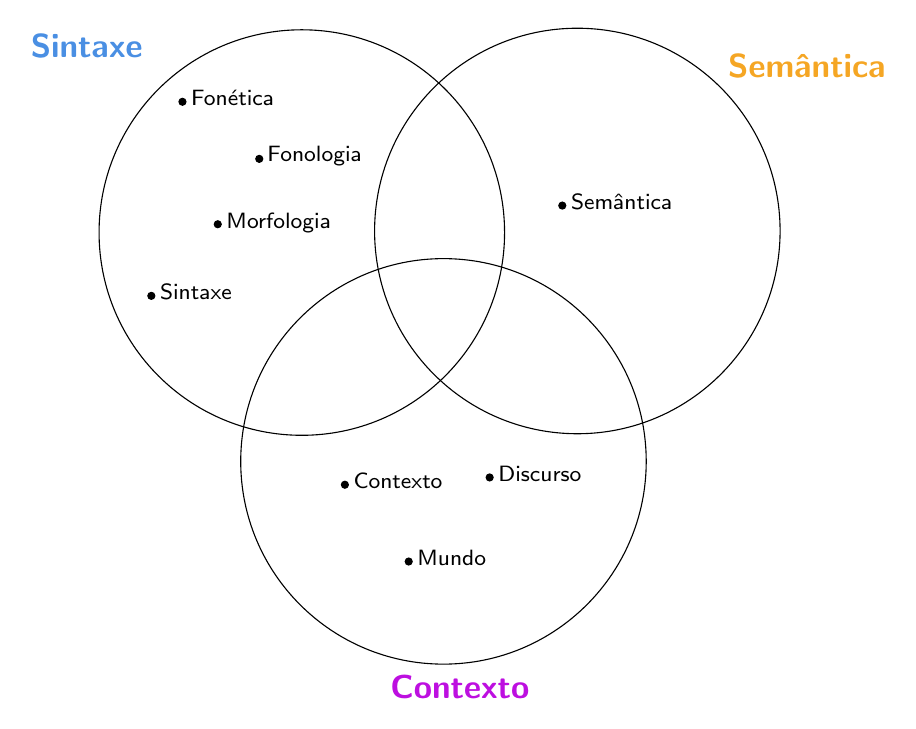
\begin{tikzpicture}[x=0.75pt,y=0.75pt,yscale=-0.75,xscale=0.75]
    %uncomment if require: \path (0,519); %set diagram left start at 0, and has height of 519
    
    %Shape: Circle [id:dp6775411490734827] 
    \draw   (75.5,169.25) .. controls (75.5,97.31) and (133.81,39) .. (205.75,39) .. controls (277.69,39) and (336,97.31) .. (336,169.25) .. controls (336,241.19) and (277.69,299.5) .. (205.75,299.5) .. controls (133.81,299.5) and (75.5,241.19) .. (75.5,169.25) -- cycle ;
    %Shape: Circle [id:dp7013179161415731] 
    \draw   (252.5,168.25) .. controls (252.5,96.31) and (310.81,38) .. (382.75,38) .. controls (454.69,38) and (513,96.31) .. (513,168.25) .. controls (513,240.19) and (454.69,298.5) .. (382.75,298.5) .. controls (310.81,298.5) and (252.5,240.19) .. (252.5,168.25) -- cycle ;
    %Shape: Circle [id:dp9236852908414266] 
    \draw   (166.5,316.25) .. controls (166.5,244.31) and (224.81,186) .. (296.75,186) .. controls (368.69,186) and (427,244.31) .. (427,316.25) .. controls (427,388.19) and (368.69,446.5) .. (296.75,446.5) .. controls (224.81,446.5) and (166.5,388.19) .. (166.5,316.25) -- cycle ;
    %Shape: Circle [id:dp8411900099296108] 
    \draw  [color={rgb, 255:red, 0; green, 0; blue, 0 }  ,draw opacity=1 ][fill={rgb, 255:red, 0; green, 0; blue, 0 }  ,fill opacity=1 ] (126.83,85.25) .. controls (126.83,84.01) and (127.84,83) .. (129.08,83) .. controls (130.33,83) and (131.33,84.01) .. (131.33,85.25) .. controls (131.33,86.49) and (130.33,87.5) .. (129.08,87.5) .. controls (127.84,87.5) and (126.83,86.49) .. (126.83,85.25) -- cycle ;
    
    %Shape: Circle [id:dp42285790681396784] 
    \draw  [color={rgb, 255:red, 0; green, 0; blue, 0 }  ,draw opacity=1 ][fill={rgb, 255:red, 0; green, 0; blue, 0 }  ,fill opacity=1 ] (176.17,121.92) .. controls (176.17,120.67) and (177.17,119.67) .. (178.42,119.67) .. controls (179.66,119.67) and (180.67,120.67) .. (180.67,121.92) .. controls (180.67,123.16) and (179.66,124.17) .. (178.42,124.17) .. controls (177.17,124.17) and (176.17,123.16) .. (176.17,121.92) -- cycle ;
    %Shape: Circle [id:dp5438038252660116] 
    \draw  [color={rgb, 255:red, 0; green, 0; blue, 0 }  ,draw opacity=1 ][fill={rgb, 255:red, 0; green, 0; blue, 0 }  ,fill opacity=1 ] (149.5,163.92) .. controls (149.5,162.67) and (150.51,161.67) .. (151.75,161.67) .. controls (152.99,161.67) and (154,162.67) .. (154,163.92) .. controls (154,165.16) and (152.99,166.17) .. (151.75,166.17) .. controls (150.51,166.17) and (149.5,165.16) .. (149.5,163.92) -- cycle ;
    
    %Shape: Circle [id:dp7047187084507844] 
    \draw  [color={rgb, 255:red, 0; green, 0; blue, 0 }  ,draw opacity=1 ][fill={rgb, 255:red, 0; green, 0; blue, 0 }  ,fill opacity=1 ] (106.83,209.92) .. controls (106.83,208.67) and (107.84,207.67) .. (109.08,207.67) .. controls (110.33,207.67) and (111.33,208.67) .. (111.33,209.92) .. controls (111.33,211.16) and (110.33,212.17) .. (109.08,212.17) .. controls (107.84,212.17) and (106.83,211.16) .. (106.83,209.92) -- cycle ;
    
    %Shape: Circle [id:dp2978376246917125] 
    \draw  [color={rgb, 255:red, 0; green, 0; blue, 0 }  ,draw opacity=1 ][fill={rgb, 255:red, 0; green, 0; blue, 0 }  ,fill opacity=1 ] (370.83,151.92) .. controls (370.83,150.67) and (371.84,149.67) .. (373.08,149.67) .. controls (374.33,149.67) and (375.33,150.67) .. (375.33,151.92) .. controls (375.33,153.16) and (374.33,154.17) .. (373.08,154.17) .. controls (371.84,154.17) and (370.83,153.16) .. (370.83,151.92) -- cycle ;
    
    %Shape: Circle [id:dp5234260157724945] 
    \draw  [color={rgb, 255:red, 0; green, 0; blue, 0 }  ,draw opacity=1 ][fill={rgb, 255:red, 0; green, 0; blue, 0 }  ,fill opacity=1 ] (231.17,331.25) .. controls (231.17,330.01) and (232.17,329) .. (233.42,329) .. controls (234.66,329) and (235.67,330.01) .. (235.67,331.25) .. controls (235.67,332.49) and (234.66,333.5) .. (233.42,333.5) .. controls (232.17,333.5) and (231.17,332.49) .. (231.17,331.25) -- cycle ;
    
    %Shape: Circle [id:dp004866918106716023] 
    \draw  [color={rgb, 255:red, 0; green, 0; blue, 0 }  ,draw opacity=1 ][fill={rgb, 255:red, 0; green, 0; blue, 0 }  ,fill opacity=1 ] (324.17,326.58) .. controls (324.17,325.34) and (325.17,324.33) .. (326.42,324.33) .. controls (327.66,324.33) and (328.67,325.34) .. (328.67,326.58) .. controls (328.67,327.83) and (327.66,328.83) .. (326.42,328.83) .. controls (325.17,328.83) and (324.17,327.83) .. (324.17,326.58) -- cycle ;
    
    %Shape: Circle [id:dp8947660528209017] 
    \draw  [color={rgb, 255:red, 0; green, 0; blue, 0 }  ,draw opacity=1 ][fill={rgb, 255:red, 0; green, 0; blue, 0 }  ,fill opacity=1 ] (272.17,380.58) .. controls (272.17,379.34) and (273.17,378.33) .. (274.42,378.33) .. controls (275.66,378.33) and (276.67,379.34) .. (276.67,380.58) .. controls (276.67,381.83) and (275.66,382.83) .. (274.42,382.83) .. controls (273.17,382.83) and (272.17,381.83) .. (272.17,380.58) -- cycle ;
    
    % Text Node
    \draw (182,112) node [anchor=north west][inner sep=0.75pt]   [align=left] {{\footnotesize Fonologia}};
    % Text Node
    \draw (133,76.33) node [anchor=north west][inner sep=0.75pt]   [align=left] {{\footnotesize Fonética}};
    % Text Node
    \draw (155.67,155) node [anchor=north west][inner sep=0.75pt]   [align=left] {{\footnotesize Morfologia}};
    % Text Node
    \draw (113,201) node [anchor=north west][inner sep=0.75pt]   [align=left] {{\footnotesize Sintaxe}};
    % Text Node
    \draw (377,143) node [anchor=north west][inner sep=0.75pt]   [align=left] {{\footnotesize Semântica}};
    % Text Node
    \draw (237.33,322.33) node [anchor=north west][inner sep=0.75pt]   [align=left] {{\footnotesize Contexto}};
    % Text Node
    \draw (330.33,317.67) node [anchor=north west][inner sep=0.75pt]   [align=left] {{\footnotesize Discurso}};
    % Text Node
    \draw (278.33,371.67) node [anchor=north west][inner sep=0.75pt]   [align=left] {{\footnotesize Mundo}};
    % Text Node
    \draw (30,40) node [anchor=north west][inner sep=0.75pt]   [align=left] {{\large \textbf{\textcolor[rgb]{0.29,0.56,0.89}{Sintaxe}}}};
    % Text Node
    \draw (478,53) node [anchor=north west][inner sep=0.75pt]   [align=left] {{\large \textbf{\textcolor[rgb]{0.96,0.65,0.14}{Semântica}}}};
    % Text Node
    \draw (261,452) node [anchor=north west][inner sep=0.75pt]   [align=left] {{\large \textbf{\textcolor[rgb]{0.74,0.06,0.88}{Contexto}}}};
    \end{tikzpicture}
    \fonte{Do autor\footnotemark}
\end{figure}

\footnotetext{Elaborada conforme sugerido por \citeonline{allen1988natural} e \citeonline{cambria2014jumping}}

Para \citeonline{allen1988natural}, além da visão sistêmica demonstrada anteriormente, há ainda um agrupamento mais específico das áreas de conhecimento relevantes ao entendimento da linguagem; para o autor, para aplicações centradas numa interação escrita, pode-se elencar como relevantes ao sistema os seguintes conhecimentos: (1) \textbf{Conhecimento Morfológico} (conhecer como as palavras são construídas no idioma ao qual o sistema busca atender - a exemplo, as palavras ferro, ferrugem e ferradura derivam todas do mesmo radical, ferr); (2) \textbf{Conhecimento Sintático} (como as palavras podem ser agrupadas, e qual o papel de cada vocábulo na estrutura construída); (3) \textbf{Conhecimento Semântico} (implica no conhecimento do significado das palavras e como estes podem ser empregadas para a construção de sentenças com significados que possuam sentido e significado, independente do contexto no qual foram empregados); (4) \textbf{Conhecimento Pragmático} (como sentenças empregadas em contextos diferentes podem assumir significados igualmente diferentes); (5) \textbf{Conhecimento do Diálogo} (como sentenças afetam umas às outras, impactando na interpretação do discurso conduzido - principalmente em relação ao emprego de pronomes e ao fluxo do diálogo ao longo do tempo); (6) \textbf{Conhecimento de Domínio} (compete ao entendimento do contexto no qual os usuários daquele domínio empregam cada vocábulo). Para aplicações cujo meio de interação com o usuário seja a voz, há a necessidade de um campo de conhecimento adicional, o \textbf{Conhecimento Fonético e Fonológico} (que se relaciona a forma como cada vocábulo relaciona-se com os sons que os representam). O relacionamento entre as áreas apresentadas pode ser melhor observado na representação vista na figura \ref{fig:M1}.


% SUBSEÇÃO 1: FUNDAMENDAÇÃO CONCEITO B----------------------------------------------------------------------------
\section{Chatbots}
\label{sec:chatbots}

Tal qual proposto por \citeonline{wezel2020m}, um \textit{chatbot} -- uma contração para o termo \textbf{robo de conversação} (do inglês, \textit{chatting robot}) \cite{lokman2018modern}, é uma aplicação baseada em diálogo, projetada para atender a uma finalidade específica e bem definida. Intentando uma expansão deste conceito, pode-se seguir a linha proposta por \citeonline{mctear2020conversational}, o qual pontua que tais sistemas são desenvolvidos para suportar interações com humanos estabelecidas de forma escrita, por fala ou mesmo por ambas as interfaces citadas; tais interações podem ser classificadas em \textbf{diálogos orientados à tarefas}, no qual o ser humano e o sistema estabelecem uma comunicação visando a completude de uma atividade qualquer, e em \textbf{diálogos não orientados a tarefas}, no qual a interação ocorre sem qualquer finalidade pré estabelecida, sendo o objetivo do sistema proporcionar àqueles que com ele interagem uma experiência póxima à comunicação rotineira obervada entre seres humanos. Esta interação é possibilitada graças à existência e à aplicação das técnicas de Processamento de Linguagem Natural \cite{lokman2018modern}.

Pode-se traçar um paralelo entre o surgimento das primeiras aplicações visando esta finalidade -- em meados da década de 1960, com o desenvolvimento da aplicação ELIZA, desenvolvida pelo MIT -- e a evolução dos estudos relacionados à disciplina de NLP \cite{lokman2018modern,allen1988natural}. Todavia, embora tenha permeado o campo computacional desde o seu surgimento, nota-se que o tema ganhou maior relevância recentemente. \citeonline{lokman2018modern} pontuam que tal eminência deve-se, principalmente, ao fato de os dispositivos celulares terem sofrido uma alteração em seu modo de operação: hoje, a troca de mensagens curtas de texto, que representa uma comunicação mais ágil e enxuta, tem-se mostrado o principal uso dos aparelhos, em detrimento à operação por voz, a qual caracteriza um meio de comunicação longo; outro fator que justificaria o recente enfoque ao tópico seria a ``corrida''  disputada pelas grandes corporações na busca de soluções no segmento de assistentes pessoais virtuais (Amazon Alexa, Google Assistant and Apple Siri) \cite{lokman2018modern}.
% SUBSEÇÃO 1: FUNDAMENDAÇÃO CONCEITO B----------------------------------------------------------------------------
\section{Aprendizado de Máquina}
\label{sec:ml}

\citeonline[tradução nossa]{alpaydin2020introduction} introduz a ideia dos \textbf{algorítimos} como o núcleo da computação, o qual pode ser definido como ``uma sequência de instruções que deve ser executada para transformar a entrada em uma saída.''\footnote{``\textit{An algorithm is a sequence of instructions that should be carried out to transform the input to an output.}''}. O autor aponta, ainda, que, desde o desenvolvimento do primeiro computador, intenta-se o desenvolvimento de algorítimos para uma grande natureza de tarefas, tornando-os indispensáveis ao meio de vida adotado pelo homem atualmente; entretanto, mesmo que peça fundamental ao cotidiano humano, ainda há, de fato, uma infinidade de tarefas que são executadas facilmente pelos seres humanos -- como reconhecer uma pessoa através de uma fotografia, atravessar uma sala cheia de pessoas ou objetos sem se chocar contra os mesmos, jogar xadrez, dirigir um carro ou estabeler e manter uma conversa numa língua estrangeira -- para as quais o desenvolvimento de um algorítimo parece virtualmente inconcebível, e para suprir tal carência é que surge o conceito de \textbf{Aprendizado de Máquina } (do inglês \textit{Machine Learning}, ou apenas \textbf{ML}) \cite{alpaydin2020introduction}.

\citeonline[tradução nossa]{michalski2013machine} declaram que ``o aprendizado é um fenômeno multifacetado. Os processos de aprendizagem incluem a aquisição de novos conhecimentos declarativos, o desenvolvimento de habilidades motoras e cognitivas através de instrução ou prática, a organização de novos conhecimentos em representações gerais e efetivas e a descoberta de novos fatos e teorias através da observação e experimentação.''\footnote{``\textit{Learning is a many-faceted phenomenon. Learning processes include the acquisition of new declarative knowledge, the development of motor and cognitive skills through instruction or practice, the organization of new knowledge into general, effective representations, and the discovery of new facts and theories through observation and experimentation}''}. Tanto \citeonline{alpaydin2020introduction} quanto \citeonline{michalski2013machine} apontam que o principal objetivo da disciplina de Aprendizado de Máquina é oferecer aos sistemas computacionais a capacidade de aprender tal qual observado no ser humano; tal afirmação é reforçada por \citeonline{el2015machine} ao escreverem que tal área de trabalho enquadra-se numa categoria de algorítmos que são capazes de emular alguns aspectos da inteligência humana. Condensando-se os conceitos anteriores, pode-se afirmar que o Aprendizado de Máquina constitui-se de capacitar a máquina da habilidade de aprender, sem que um ser humano a tenha programado explicitamente \cite{samuel1988some}.

            	    	% Fundamentação Teórica
% %CRONOGRAMA------------------------------------------------------------------------------------------------------
\chapter{CRONOGRAMA}
\label{chap:cronograma}

% Please add the following required packages to your document preamble:
% \usepackage{booktabs}
% \usepackage[table,xcdraw]{xcolor}
% If you use beamer only pass "xcolor=table" option, i.e. \documentclass[xcolor=table]{beamer}
\begin{table}[!htb]
    \begin{tabular}{@{}llllllll@{}}
    \toprule
    \rowcolor[HTML]{EFEFEF} 
    \textbf{Etapa Proposta}                                                                                      & \textbf{Jun}             & \textbf{Jul}             & \textbf{Ago}             & \textbf{Set}             & \textbf{Out}             & \textbf{Nov}             & \textbf{Dez}             \\ \midrule
    Levantamento de Bibiografia                                                                                  & {\color[HTML]{656565} X} & {\color[HTML]{656565} }  & {\color[HTML]{656565} }  & {\color[HTML]{656565} }  & {\color[HTML]{656565} }  & {\color[HTML]{656565} }  & {\color[HTML]{656565} }  \\
    Condensação do Material                                                                                      & {\color[HTML]{656565} X} & {\color[HTML]{656565} }  & {\color[HTML]{656565} }  & {\color[HTML]{656565} }  & {\color[HTML]{656565} }  & {\color[HTML]{656565} }  & {\color[HTML]{656565} }  \\
    \begin{tabular}[c]{@{}l@{}}Leitura e Fichamento do Material;\\ Redação da Fundamentação Teórica\end{tabular} & {\color[HTML]{656565} }  & {\color[HTML]{656565} X} & {\color[HTML]{656565} }  & {\color[HTML]{656565} }  & {\color[HTML]{656565} }  & {\color[HTML]{656565} }  & {\color[HTML]{656565} }  \\
    Aquisição da Base de Dados                                                                                   & {\color[HTML]{656565} }  & {\color[HTML]{656565} }  & {\color[HTML]{656565} X} & {\color[HTML]{656565} }  & {\color[HTML]{656565} }  & {\color[HTML]{656565} }  & {\color[HTML]{656565} }  \\
    Desenvolvimento da Aplicação de Chatbot                                                                      & {\color[HTML]{656565} }  & {\color[HTML]{656565} }  & {\color[HTML]{656565} }  & {\color[HTML]{656565} X} & {\color[HTML]{656565} X} & {\color[HTML]{656565} }  & {\color[HTML]{656565} }  \\
    Testes e Observação de Resultado                                                                             & {\color[HTML]{656565} }  & {\color[HTML]{656565} }  & {\color[HTML]{656565} }  & {\color[HTML]{656565} }  & {\color[HTML]{656565} X} & {\color[HTML]{656565} }  & {\color[HTML]{656565} }  \\
    Revisão do Texto/Redação Final                                                                               & {\color[HTML]{656565} }  & {\color[HTML]{656565} }  & {\color[HTML]{656565} }  & {\color[HTML]{656565} }  & {\color[HTML]{656565} }  & {\color[HTML]{656565} X} & {\color[HTML]{656565} }  \\
    Apresentação para a Banca Examinadora                                                                        & {\color[HTML]{656565} }  & {\color[HTML]{656565} }  & {\color[HTML]{656565} }  & {\color[HTML]{656565} }  & {\color[HTML]{656565} }  & {\color[HTML]{656565} }  & {\color[HTML]{656565} X} \\ \bottomrule
    \end{tabular}
\end{table}

% SUBSEÇÕES DE FUNDAMENTAÇÃO--------------------------------------------------------------------------------------
% Descomente as linhas abaixo caso deseje estruturar seu capítulo em seções; outras seções podem ser criadas utilizando-se as fornecidas como modelo.
%% SUBSEÇÃO 1: OBJETIVO GERAL--------------------------------------------------------------------------------------
\section{OBJETIVO GERAL}
\label{sec:objetivo_geral}

Criar uma solução baseada em \textit{chatbots}, a qual sirva como ferramenta auxiliar no preenchimento de documentos relacionados ao setor de comércio exterior, focando na atividade de importação.
%\section{OBJETIVOS ESPECÍFICOS}
\label{sec:objetivos_especificos}

\begin{itemize}
    \item Coletar os dados e metadados de perfis de usuários do Twitter relacionados aos possíveis presidenciáveis;
    \item Consolidar os registros obtidos em uma base de dados modelada usando o princípio de seguidores recíprocos;
    \item Identificar os termos associados a cada grupo representado pelos pré-candidatos;
    \item Processar a base de dados construída com o uso de técnicas de NLP e modelos de classificação;
    \item Aplicar o LIME em cima do modelo de classificação empregado;
    \item Construir um panorama da distribuição dos usuários do Twitter em relação ao seu posicionamento político considerando possíveis candidatos à presidência e os termos identificadores elencados.
\end{itemize}


              	     	% Metodologia
% %CRONOGRAMA------------------------------------------------------------------------------------------------------
\chapter{CRONOGRAMA}
\label{chap:cronograma}

% Please add the following required packages to your document preamble:
% \usepackage{booktabs}
% \usepackage[table,xcdraw]{xcolor}
% If you use beamer only pass "xcolor=table" option, i.e. \documentclass[xcolor=table]{beamer}
\begin{table}[!htb]
    \begin{tabular}{@{}llllllll@{}}
    \toprule
    \rowcolor[HTML]{EFEFEF} 
    \textbf{Etapa Proposta}                                                                                      & \textbf{Jun}             & \textbf{Jul}             & \textbf{Ago}             & \textbf{Set}             & \textbf{Out}             & \textbf{Nov}             & \textbf{Dez}             \\ \midrule
    Levantamento de Bibiografia                                                                                  & {\color[HTML]{656565} X} & {\color[HTML]{656565} }  & {\color[HTML]{656565} }  & {\color[HTML]{656565} }  & {\color[HTML]{656565} }  & {\color[HTML]{656565} }  & {\color[HTML]{656565} }  \\
    Condensação do Material                                                                                      & {\color[HTML]{656565} X} & {\color[HTML]{656565} }  & {\color[HTML]{656565} }  & {\color[HTML]{656565} }  & {\color[HTML]{656565} }  & {\color[HTML]{656565} }  & {\color[HTML]{656565} }  \\
    \begin{tabular}[c]{@{}l@{}}Leitura e Fichamento do Material;\\ Redação da Fundamentação Teórica\end{tabular} & {\color[HTML]{656565} }  & {\color[HTML]{656565} X} & {\color[HTML]{656565} }  & {\color[HTML]{656565} }  & {\color[HTML]{656565} }  & {\color[HTML]{656565} }  & {\color[HTML]{656565} }  \\
    Aquisição da Base de Dados                                                                                   & {\color[HTML]{656565} }  & {\color[HTML]{656565} }  & {\color[HTML]{656565} X} & {\color[HTML]{656565} }  & {\color[HTML]{656565} }  & {\color[HTML]{656565} }  & {\color[HTML]{656565} }  \\
    Desenvolvimento da Aplicação de Chatbot                                                                      & {\color[HTML]{656565} }  & {\color[HTML]{656565} }  & {\color[HTML]{656565} }  & {\color[HTML]{656565} X} & {\color[HTML]{656565} X} & {\color[HTML]{656565} }  & {\color[HTML]{656565} }  \\
    Testes e Observação de Resultado                                                                             & {\color[HTML]{656565} }  & {\color[HTML]{656565} }  & {\color[HTML]{656565} }  & {\color[HTML]{656565} }  & {\color[HTML]{656565} X} & {\color[HTML]{656565} }  & {\color[HTML]{656565} }  \\
    Revisão do Texto/Redação Final                                                                               & {\color[HTML]{656565} }  & {\color[HTML]{656565} }  & {\color[HTML]{656565} }  & {\color[HTML]{656565} }  & {\color[HTML]{656565} }  & {\color[HTML]{656565} X} & {\color[HTML]{656565} }  \\
    Apresentação para a Banca Examinadora                                                                        & {\color[HTML]{656565} }  & {\color[HTML]{656565} }  & {\color[HTML]{656565} }  & {\color[HTML]{656565} }  & {\color[HTML]{656565} }  & {\color[HTML]{656565} }  & {\color[HTML]{656565} X} \\ \bottomrule
    \end{tabular}
\end{table}

% SUBSEÇÕES DE FUNDAMENTAÇÃO--------------------------------------------------------------------------------------
% Descomente as linhas abaixo caso deseje estruturar seu capítulo em seções; outras seções podem ser criadas utilizando-se as fornecidas como modelo.
%% SUBSEÇÃO 1: OBJETIVO GERAL--------------------------------------------------------------------------------------
\section{OBJETIVO GERAL}
\label{sec:objetivo_geral}

Criar uma solução baseada em \textit{chatbots}, a qual sirva como ferramenta auxiliar no preenchimento de documentos relacionados ao setor de comércio exterior, focando na atividade de importação.
%\section{OBJETIVOS ESPECÍFICOS}
\label{sec:objetivos_especificos}

\begin{itemize}
    \item Coletar os dados e metadados de perfis de usuários do Twitter relacionados aos possíveis presidenciáveis;
    \item Consolidar os registros obtidos em uma base de dados modelada usando o princípio de seguidores recíprocos;
    \item Identificar os termos associados a cada grupo representado pelos pré-candidatos;
    \item Processar a base de dados construída com o uso de técnicas de NLP e modelos de classificação;
    \item Aplicar o LIME em cima do modelo de classificação empregado;
    \item Construir um panorama da distribuição dos usuários do Twitter em relação ao seu posicionamento político considerando possíveis candidatos à presidência e os termos identificadores elencados.
\end{itemize}


	              	     	% Cronograma

\postextual
% INSERE ELEMENTOS PÓS-TEXTUAIS
% REFERÊNCIAS------------------------------------------------------------------

% Carrega o arquivo "base-referencias.bib" e extrai automaticamente as referências citadas

\bibliography{./base-referencias}
\bibliographystyle{abntex2-alf} % Define o estilo ABNT para formatar a lista de referências
% OBSERVAÇÕES------------------------------------------------------------------
% Este arquivo não precisa ser alterado.
           			           	% Referências
%% APÊNDICES--------------------------------------------------------------------

\begin{apendicesenv}
\partapendices

% Primeiro apêndice------------------------------------------------------------
\chapter{Nome do apêndice} % Edite para alterar o título deste apêndice
\label{chap:apendiceA}

Lembre-se que a diferença entre apêndice e anexo diz respeito à autoria do texto e/ou material ali colocado.

Caso o material ou texto suplementar ou complementar seja de sua autoria, então ele deverá ser colocado como um apêndice. Porém, caso a autoria seja de terceiros, então o material ou texto deverá ser colocado como anexo.

Caso seja conveniente, podem ser criados outros apêndices para o seu trabalho acadêmico. Basta recortar e colar este trecho neste mesmo documento. Lembre-se de alterar o "label"{} do apêndice.

Não é aconselhável colocar tudo que é complementar em um único apêndice. Organize os apêndices de modo que, em cada um deles, haja um único tipo de conteúdo. Isso facilita a leitura e compreensão para o leitor do trabalho.

% Novo apêndice----------------------------------------------------------------
\chapter{Nome do outro apêndice}
\label{chap:apendiceB}

conteúdo do novo apêndice

\end{apendicesenv}
             				   	% Apêndices
%% ANEXO------------------------------------------------------------------------

\begin{anexosenv}
\partanexos

% Primeiro anexo---------------------------------------------------------------
\chapter{Nome do anexo}     % edite para alterar o título deste anexo
\label{chap:anexoA}

Lembre-se que a diferença entre apêndice e anexo diz respeito à autoria do texto e/ou material ali colocado.

Caso o material ou texto suplementar ou complementar seja de sua autoria, então ele deverá ser colocado como um apêndice. Porém, caso a autoria seja de terceiros, então o material ou texto deverá ser colocado como anexo.

Caso seja conveniente, podem ser criados outros anexos para o seu trabalho acadêmico. Basta recortar e colar este trecho neste mesmo documento. Lembre-se de alterar o "label"{} do anexo.

Organize seus anexos de modo a que, em cada um deles, haja um único tipo de conteúdo. Isso facilita a leitura e compreensão para o leitor do trabalho. É para ele que você escreve.

% Novo anexo-------------------------------------------------------------------
\chapter{Nome do outro anexo}
\label{chap:anexoB}

conteúdo do outro anexo

\end{anexosenv}
               					   	% Anexos

\end{document}
